\documentclass{article}     %type of document
\usepackage[utf8]{inputenc} %for text encoding
\usepackage[italian]{babel} %for language elements
\usepackage{graphicx}   %for adding figures
\usepackage[a4paper, portrait, margin=2cm]{geometry}   %paper shape
%\usepackage{listings}       %displays code
%\usepackage{subcaption}     %for subfigures

\title{Verifica di Laboratorio di Matematica}
\author{Davide Borra }
\date{Dicembre 2020}

\begin{document}

\maketitle
\begin{abstract}
    Nella seguente prova si chiede allo studente di individuare un elemento della vita dei tutti i giorni che segua un modello periodico riconducibile ad una funzione sinusoidale e produrre un esercizio simile a quelli svolti in classe in merito al fenomeno individuato. Lo studente dovrà poi svolgere l'esercizio.
\end{abstract}

\section*{Consegna}
    Si consideri un sistema costituito da un carrello ad attrito trascurabile posto su una rotaia e collegato a due molle. Esso viene messo in movimento e i sensori posti sul carrello rilevano la posizione dello stesso a partire dell'inizio della rotaia. I dati sono riportati nella tabella seguente:
    
    \vspace{0.2 cm}
    \begin{tabular}{|c|c|}
        \hline
        $t (s)$ & $y (m)$\\ \hline \hline
        0,1 & 0,52 \\ \hline
        0,2 & 0,71 \\ \hline
        0,3 & 0,86 \\ \hline
        0,4 & 0,92 \\ \hline
        0,5 & 0,89 \\ \hline
        0,6 & 0,78 \\ \hline
        0,7 & 0,60 \\ \hline
        0,8 & 0,40 \\ \hline
        0,9 & 0,23 \\ \hline
        1,0 & 0,11 \\ \hline
        1,1 & 0,09 \\ \hline
        1,2 & 0,15 \\ \hline
        1,4 & 0,29 \\ \hline
        1,4 & 0,48 \\ \hline
    \end{tabular}
    \vspace{0.2 cm}
    
    Sapendo che il carrello si muove di moto armonico e che segue quindi un modello rappresentabile con una funzione del tipo $y=A\cdot \sin(\omega t + \varphi)+B$, svolgere le seguenti consegne:
    \begin{enumerate}
        \item Si rappresentino i dati utilizzando il software GeoGebra e si alleghi lo \textit{screenshot} delle viste grafici, algebra e foglio di calcolo.
        \item Si determini con carte e penna una funzione sinusoidale che ben approssimi ai dati forniti riportandone l'espressione analitica e specificando come sono stati ottenuti i valori di $B$, $T$, $|A|$, $\varphi$, $\omega$ \label{item: cartaEPenna}
        \item Si stimi, in base al modello del punto \ref{item: cartaEPenna} il la posizione del carrello nell'istante $t=1,05 s$
        \item Si determini mediante gli strumenti messi a disposizione da GeoGebra una funzione sinusoidale che si adatti bene ai dati forniti e se ne riporti l'espressione analitica.
        \item Sapendo che il carrellino nell'istante $t=1,05 s$ si trovava ad una distanza $y= 0,09 m$ dall'inizio della rotaia, quale dei due modelli costruiti consente una previsione migliore? Si motivi la risposta. Si supporti la propria analisi anche mediante il calcolo dell'indice quadratico relativo. Si alleghi il foglio di calcolo utilizzato per lo svolgimento dell'esercizio. 
    \end{enumerate}
    
\section*{Svolgimento}
\subsection*{1.}
    Tramite l'inserimento dei dati nella vista "foglio di calcolo" e l'utilizzo del comando "lista di punti" si ottiene la seguente rappresentazione:
    
    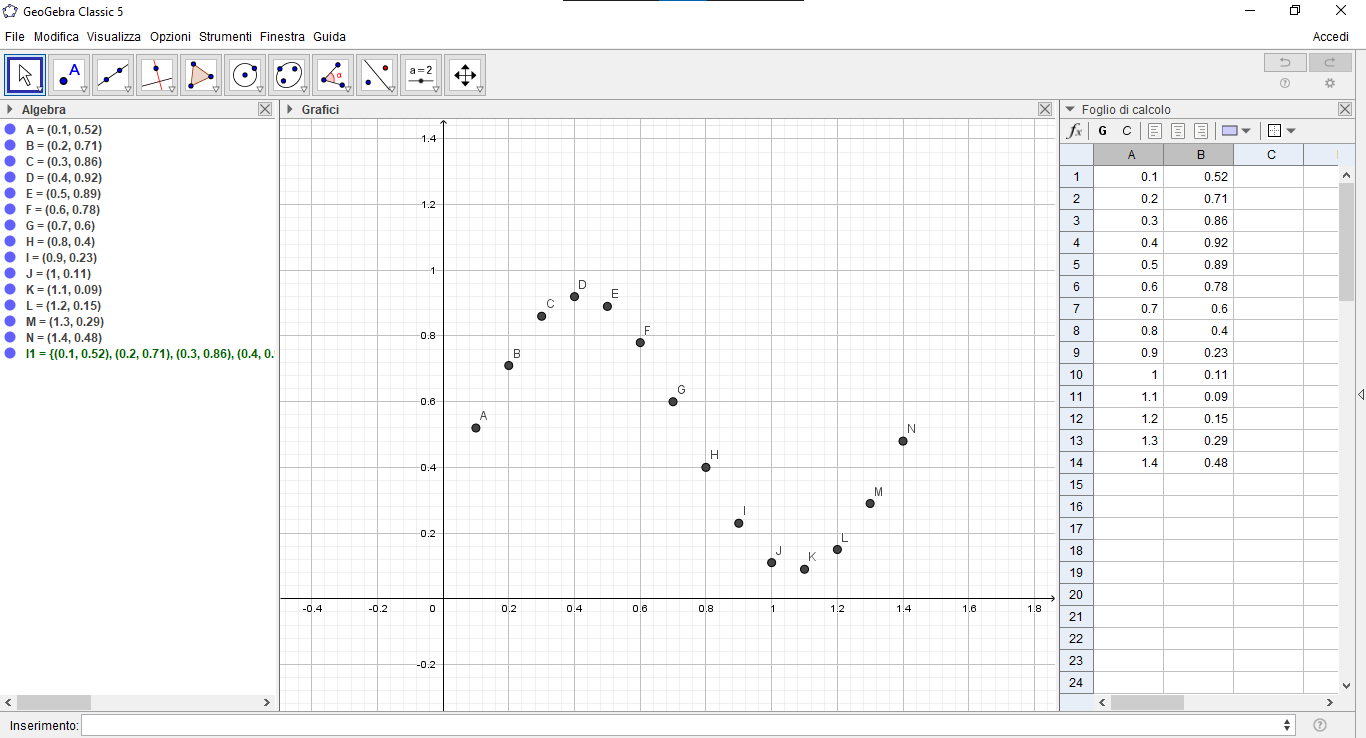
\includegraphics[width = 0.9\textwidth]{1.png}

\subsection*{2.}
    \[B = \frac{y_{max}+y_{min}}{2} = \frac{0,92 m+0,09 m}{2} = 0,51 m\]
    \[|A| = \frac{|y_{max}-y_{min}|}{2} = \frac{|0,92 m-0,09 m|}{2} = |0,42 m| = 0,42 m\]
    \[T = 1,3 s\] Ricavato dalla differenza tra gli istanti corrispondenti ai due estremi nella rappresentazione grafica
    \[\omega = \frac{2\pi}{T}=\frac{2\pi}{1,3s} = \frac{20}{13}\pi Hz\]
    
    Il valore di $\varphi$ si ricava in via grafica tramite la rappresentazione della funzione su GeoGebra e la sostituzione di uno \textit{slider} al posto della variabile cercata, da cui si ottiene $\varphi = -0,5$. 
    Da ciò si ottiene la funzione sinusoidale
    \[y=0,42 \cdot \sin \left( \frac{20}{13} \pi \cdot t -0,5 \right)+0,51 \]
\subsection*{3.}
    Sostituendo nell'equazione individuata al punto precedente il valore di $t=1,05s$, si ottiene:
    \[y=0,42 \cdot \sin \left( \frac{20}{13} \pi \cdot 1,05 -0,5 \right)+0,51 = 0,09m\]
\subsection*{4.}
    Tramite il comando di GeoGebra \texttt{RegSin()} è possibile determinare una funzione che approssimi bene il modello descritto. Inserendo quindi il comando citato, si ricava la seguente funzione:
    \[y=0,5+0,42\cdot\sin\left(4,76\cdot t-0,43\right)\]
    
\subsection*{5.}
    Sostituendo il valore di $t=1,05 s$ nell'equazione determinata al punto precedente si ottiene: 
    \[y=0,5+0,42\cdot\sin\left(4,76\cdot 1,05 -0,43\right)=0,09m\]
    Entrambi i valori ottenuti sono quindi corretti. Questo metodo non permette quindi di determinare la funzione che approssima meglio i dati considerati. Ciò è dovuto alla grande quantità di valori considerati (il che aiuta ad avere un'approssimazione maggiore) e, conseguentemente, al fatto che le due funzioni siano particolarmente simili. Per determinare il modello migliore è quindi necessario utilizzare un foglio di calcolo (nel mio caso Microsoft Office Excel 2019) per calcolare l'indice quadratico medio $I_2$.
    
    Tramite i calcoli effettuati utilizzando il foglio di calcolo allegato si ottengono i seguenti valori, dove $I_{2,M}$ è riferito alla funzione determinata con carta e penna e $I_{2,S}$ è riferito alla funzione determinata tramite GeoGebra:
    
    \[I_{2,M}=\frac{\sqrt{\frac{\sum(\hat{y}_i-y_i)^2}{N}}}{\frac{\sum\hat{y}_i}{N}} = 0,026913465\]
    
    \[I_{2,S}=\frac{\sqrt{\frac{\sum(\hat{y}_i-y_i)^2}{N}}}{\frac{\sum\hat{y}_i}{N}} = 0,007141035\]
    
    Dove con $y_i$ si intendono i valori osservati (contenuti nella tabella iniziale) mentre con $\hat{y}_i$ si intendono i valori previsti dal modello considerato.
    
    Siccome $I_{2,S} < I_{2,M}$ la previsione fornita da GeoGebra è migliore di quella fatta con carta e penna. Inoltre, siccome sia $I_{2,S} \ll 1$ che $I_{2,M} \ll 1$, entrambi i modelli sono da ritenersi validi a causa delle osservazioni fatte in precedenza.
\end{document}
